\documentclass{article}
\usepackage{graphicx}
\usepackage{fancyhdr}
\usepackage{wrapfig}
\usepackage{subcaption}
\usepackage[margin=1.5in]{geometry}
% Introduction and background (1 page)
% Literature review (1/2 page)
% Dataset Description and exploratory data analysis of the dataset (1-2 page)
% Proposed methodology (1 page)
% Experimental results (2-3 pages)
% Conclusion and discussion -- you can include the project roadmap here too (1/2 page)
% References (no limit)
\linespread{1}
\pagestyle{fancy}
\title{\textbf{Credit Score Classification}}
\author{Kyle Jow, Jimmy Nguyen, Kyle Pickle, Jacob Tuttle, Kris Wong}
\date{December 2023}

\begin{document}
\pagenumbering{gobble}
\maketitle
\newpage
\pagenumbering{arabic}
\pagestyle{fancy}
\fancyhf{} % clear header and footer
\fancyhead[R]{Credit Score Classification}
\fancyfoot[R]{\thepage}
\section*{Introduction and background}
A common problem in the finance and banking industry is assessing the risk involved with lending money to clients.
To better assess a borrower's creditworthiness, lenders formulate and assign “credit scores” to their clients, based on preconceived data 
like income, spending, and credit history.
This score can then be used by a bank as an indicator of whether a client will default or otherwise miss a payment on a given loan.
The rise of cloud-based computing in the 21st century has made it more advantageous and easier than ever for banks to share a
standardized database of credit scores and financial information on their clients.
As a result, credit scoring is being used more and more frequently to determine “worthiness” for almost anything -- qualifying for
mortgages, insurance, and even more nuanced decisions like cell phone plans and determining your employability.
\vspace{5mm}\newline
With this increase in credit scoring has come an increased interest in financial literacy among clients as to how to understand and improve
one's score.
As such, credit standards like FICO and VantageScore have begun giving their clients a way to view an estimation of their credit score, often
provided through the bank and credit card services that utilize them.
These credit score estimates are predicted in a way that is simple for the client to understand, often broken down into categories like
“poor,” “standard,” and “good” and presented alongside graphs displaying factors like age bracket and income to put them into perspective.
This demand for straightforward and transparent credit scoring by governments and clients alike has interestingly compelled banks to
consider less intricate or “black box” machine learning models, creating a delicate balance between accuracy and simplicity.
\vspace{5mm}\newline
credit scoring has always been a common, concrete example of machine learning, as -- in the world of economics -- even the tiniest increase
in accuracy can save billions of dollars in the long-run.
As a result, researchers have utilized a variety of machine learning algorithms to better predict credit scores and risk.
Nearly all client data is now digitized by banks, and with numerous complex variables that drive one's score, credit score prediction
through machine learning is an ideal way to not only predict creditworthiness but constantly tune the equations and hyperparameters used
to determine it in the midst of a fluctuating, real-world economy.

% \newpage
\section*{Literature review}
Economists and researchers alike have utilized a variety of machine learning algorithms to predict credit scores and investment risk.
Some common examples include decision trees, logistic regression, and Support Vector Machines (SVM).
\vspace{5mm}\newline
% https://www.sciencedirect.com/science/article/pii/S1568494620302039
With the history of credit scoring tracing its roots back to the 1950s, bank decisions were initially guided by the
5 C's approach -- Character, Capital, Collateral, Capacity, and Condition -- relying on subjective, physically-recorded information it its
assessments.
While we could now consider this approach a decision-tree model, Dastile et al. describe how the financial industry's regulatory need for
transparency in lending decisions has led to the prevalence of logistic regression models, known for their simplicity and interpretability.
While sophisticated, higher-accuracy machine learning models have arisen over time, their opacity continues to raise concerns.
In response, Dastile et al. go on to note several key machine learning techniques between 2010 and 2018 that have created a guided
framework of credit scoring, combining both accuracy and transparency in lending decisions.
\vspace{5mm}\newline
% https://www.sciencedirect.com/science/article/pii/S0377221721005695#sec0012
One modern approach to credit scoring comes from Dumitrescu et. al., who use a particular model called Penalised Logistic Tree Regression
(PLTR) for credit score classification with an improved logistic regression model that has non-linear decision tree effects.
It is able to predict credit score more accurately than the benchmark logistic regression commonly used in the industry, and on a level
that is comparable to more accurate random forest models.
This is because it is able to capture recursive, multi-variable traits in the data unnoticed by a typical logistic regression.
Dumitrescu et. al. use multiple datasets to test the robustness of the model and argue that PLTR preserves the needed transparency and
interpretability that come with logistic regression.

\newpage
\section*{Dataset description and exploratory data analysis}
The dataset contains 27 features. The features we will be focusing on in order
to classify a person's credit score, which is categorical, into either ``good", ``standard", or ``poor" credit
will be features that had the most correlation with credit score according to the heat map
generated from this data and features used in real-life credit score assessing. Although the Credit\_Utilization\_Ratio has little 
correlation to credit score, this feature is used to assess credit in real life, so we kept it. (Figure 1).\\
\begin{figure}[h]
    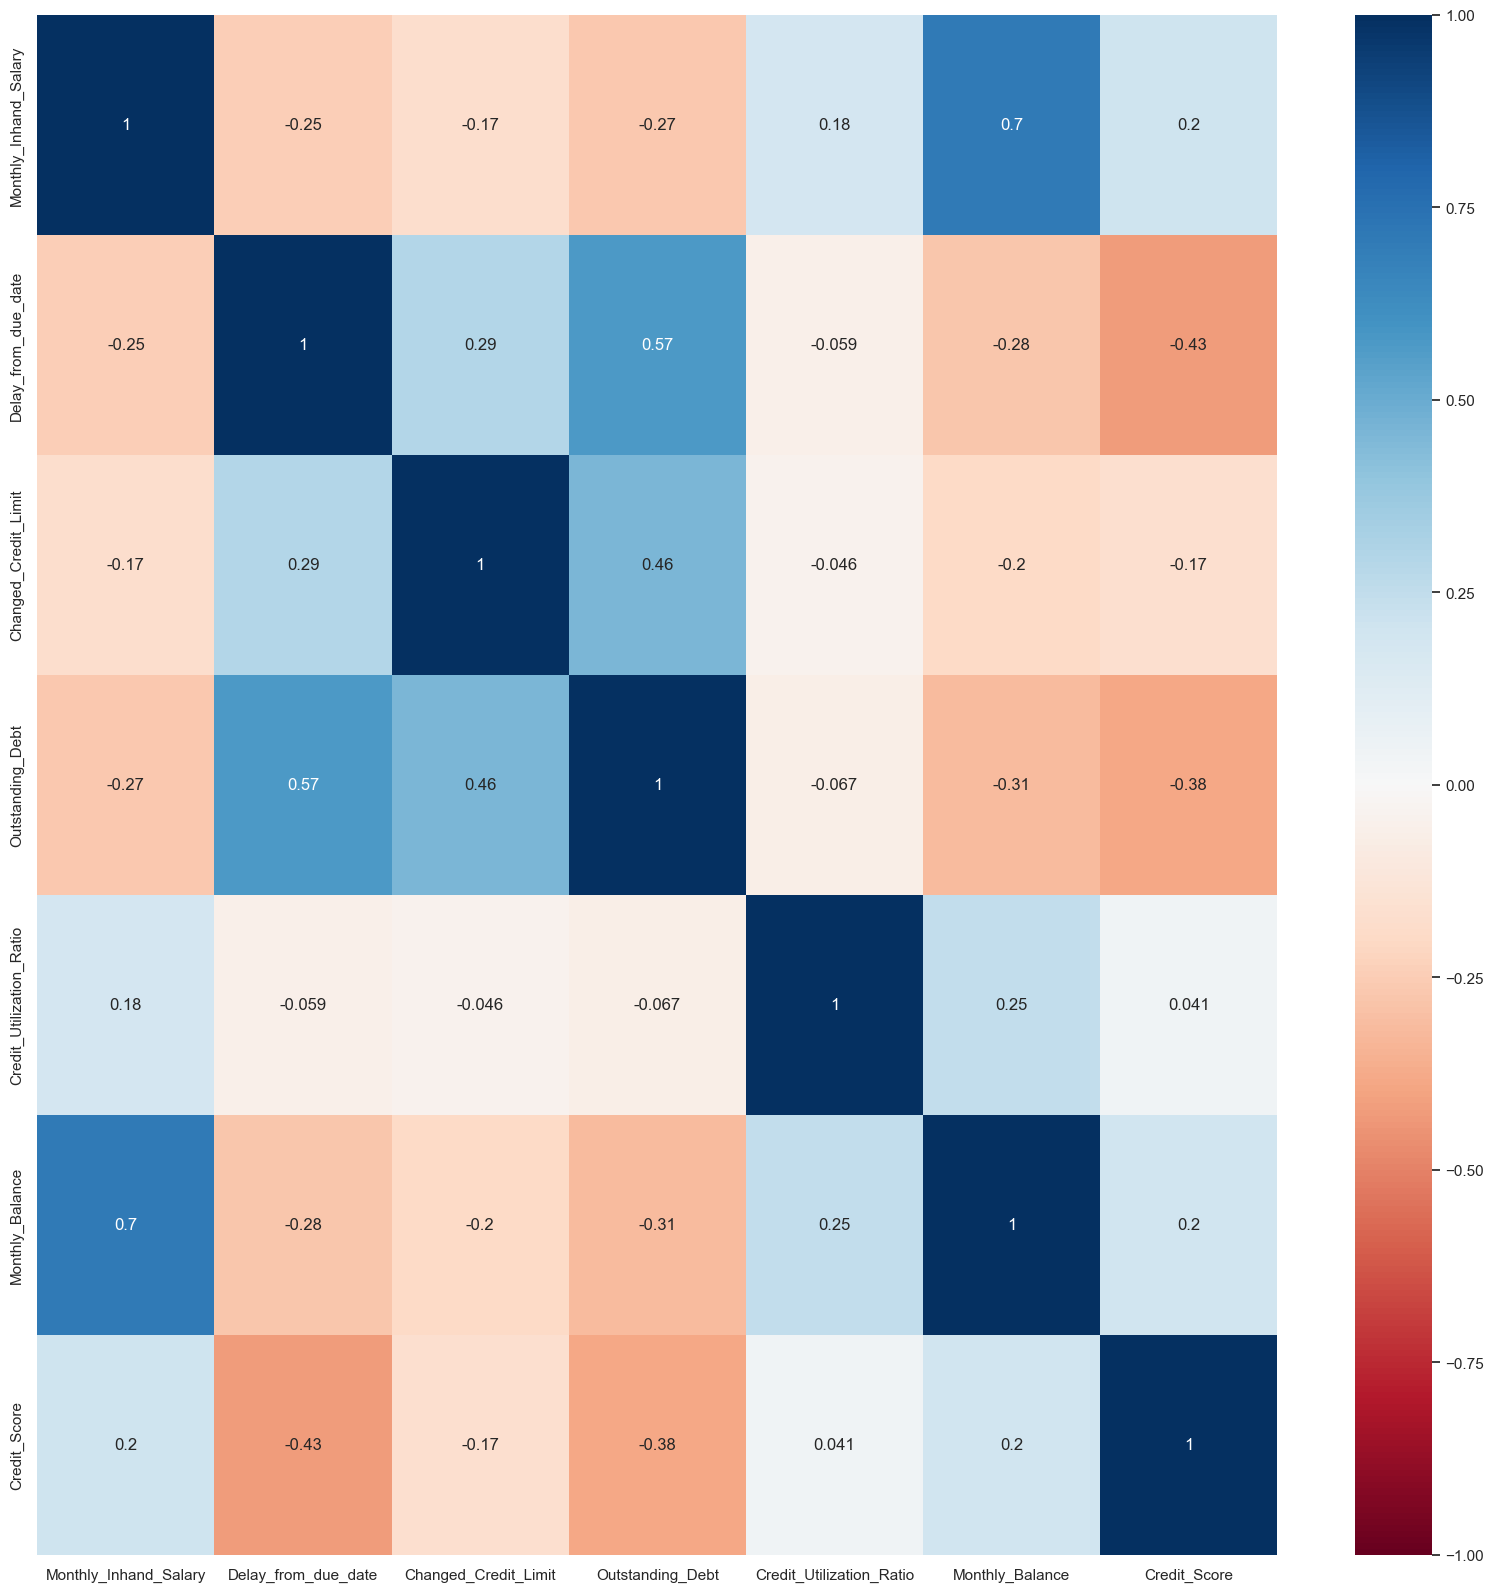
\includegraphics[width=\textwidth]{credscoreheatmap.png}
    \caption{Heat map correlation.}
    \label{fig:figure1}
\end{figure}
\newpage
\section*{Proposed methodology}
From the literature review and the fact that this problem involves multiclassification,
we decided to make and compare two SVM models with a linear and RBF kernel and one 
multinomial logistic regression model. Additionally, we used Streamlit to host our model online.


\section*{Experimental results}
Below are the classification reports for each of the models:\\
\begin{table}[!ht]
    \centering
    \begin{tabular}{|l|l|l|l|l|}
    \hline
        % RBF Kernel & ~ & ~ & ~ & ~ \\ \hline
        ~ & precision & recall & f1-score & support \\ \hline
        ~ & ~ & ~ & ~ & ~ \\ \hline
        1 & 0.7 & 0.48 & 0.57 & 2774 \\ \hline
        2 & 0.6 & 0.88 & 0.72 & 5064 \\ \hline
        3 & 0.56 & 0.02 & 0.05 & 1565 \\ \hline
        ~ & ~ & ~ & ~ & ~ \\ \hline
        accuracy & ~ & ~ & 0.62 & 9403 \\ \hline
        macro avg & 0.62 & 0.46 & 0.44 & 9403 \\ \hline
        weighted avg & 0.62 & 0.62 & 0.56 & 9403 \\ \hline
    \end{tabular}
    \caption{Classification report for SVM with RBF kernel}
\end{table}
\begin{table}[!ht]
    \centering
    \begin{tabular}{|l|l|l|l|l|}
    \hline
        % Linear Kernel & ~ & ~ & ~ & ~ \\ \hline
        ~ & precision & recall & f1-score & support \\ \hline
        ~ & ~ & ~ & ~ & ~ \\ \hline
        1 & 0.62 & 0.41 & 0.5 & 2774 \\ \hline
        2 & 0.58 & 0.87 & 0.7 & 5064 \\ \hline
        3 & 0 & 0 & 0 & 1565 \\ \hline
        ~ & ~ & ~ & ~ & ~ \\ \hline
        accuracy & ~ & ~ & 0.59 & 9403 \\ \hline
        macro avg & 0.4 & 0.43 & 0.4 & 9403 \\ \hline
        weighted avg & 0.5 & 0.59 & 0.52 & 9403 \\ \hline
    \end{tabular}
    \caption{Classification report for SVM with linear kernel}
\end{table}
\begin{table}[!ht]
    \centering
    \begin{tabular}{|l|l|l|l|l|}
    \hline
        % Logistic w/ outliers & ~ & ~ & ~ & ~ \\ \hline
        ~ & precision & recall & f1-score & support \\ \hline
        ~ & ~ & ~ & ~ & ~ \\ \hline
        1 & 0.63 & 0.42 & 0.5 & 4317 \\ \hline
        2 & 0.59 & 0.82 & 0.69 & 8022 \\ \hline
        3 & 0.47 & 0.17 & 0.25 & 2632 \\ \hline
        ~ & ~ & ~ & ~ & ~ \\ \hline
        accuracy & ~ & ~ & 0.59 & 14971 \\ \hline
        macro avg & 0.56 & 0.47 & 0.48 & 14971 \\ \hline
        weighted avg & 0.58 & 0.59 & 0.56 & 14971 \\ \hline
    \end{tabular}
    \caption{Classification report for logistic model with outliers}
\end{table}
\begin{table}[!ht]
    \centering
    \begin{tabular}{|l|l|l|l|l|}
    \hline
        % Logistic w/o outliers & ~ & ~ & ~ & ~ \\ \hline
        ~ & precision & recall & f1-score & support \\ \hline
        ~ & ~ & ~ & ~ & ~ \\ \hline
        1 & 0.6 & 0.37 & 0.45 & 3483 \\ \hline
        2 & 0.61 & 0.81 & 0.69 & 7642 \\ \hline
        3 & 0.5 & 0.29 & 0.36 & 2719 \\ \hline
        ~ & ~ & ~ & ~ & ~ \\ \hline
        accuracy & ~ & ~ & 0.59 & 13844 \\ \hline
        macro avg & 0.57 & 0.49 & 0.5 & 13844 \\ \hline
        weighted avg & 0.58 & 0.59 & 0.57 & 13844 \\ \hline
    \end{tabular}
    \caption{Classification report for logistic model with no outliers}
\end{table}
\pagebreak
\begin{figure}[!htpb]
\begin{subfigure}{0.49\textwidth}
    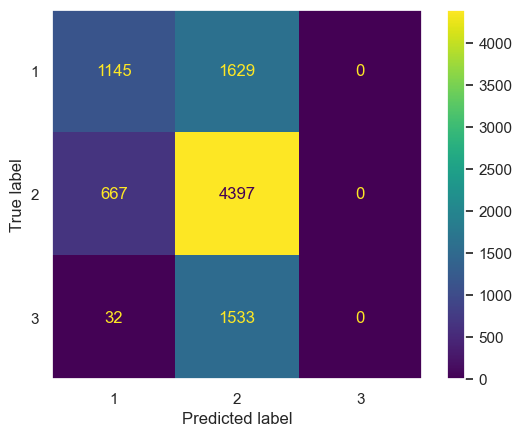
\includegraphics[width=\textwidth]{svmli.png}
    \caption{SVM, linear kernel}
    % 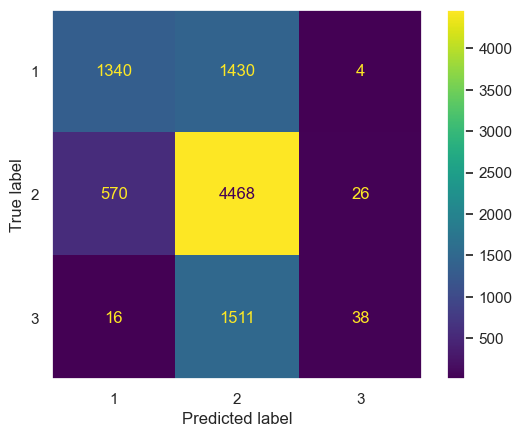
\includegraphics[width=0.5\textwidth]{svmrbf.png}
    % \caption{Confusion matrix for SVM, RBF kernel.}
    % \label{fig:left}
\end{subfigure}
\begin{subfigure}{0.49\textwidth}
    % 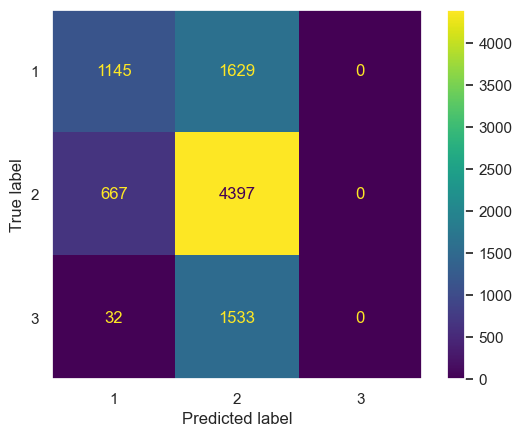
\includegraphics[width=\textwidth]{svmli.png}
    % \caption{Confusion matrix for SVM, linear kernel.}
    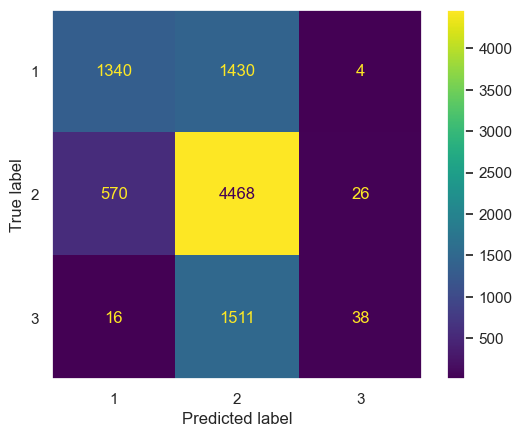
\includegraphics[width=\textwidth]{svmrbf.png}
    \caption{SVM, RBF kernel}
    % \label{fig:right}
\end{subfigure}
\begin{subfigure}{0.49\textwidth}
    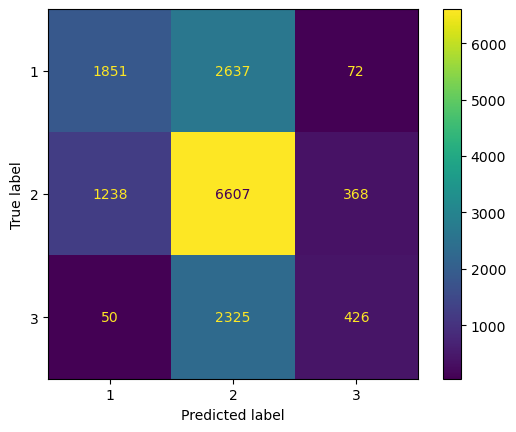
\includegraphics[width=\textwidth]{logisticNoOutliers.png}
    \caption{Logistic with no outliers}
    % 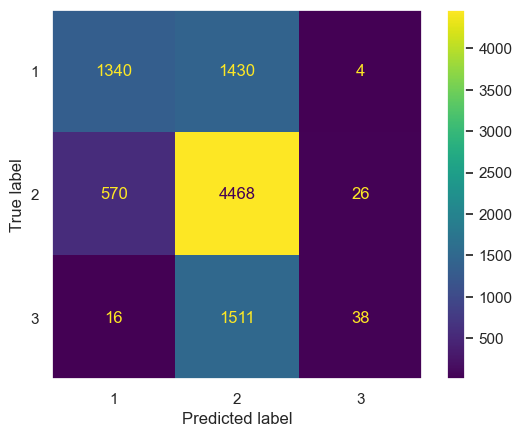
\includegraphics[width=0.5\textwidth]{svmrbf.png}
    % \caption{Confusion matrix for SVM, RBF kernel.}
    % \label{fig:left}
\end{subfigure}
\begin{subfigure}{0.49\textwidth}
    % 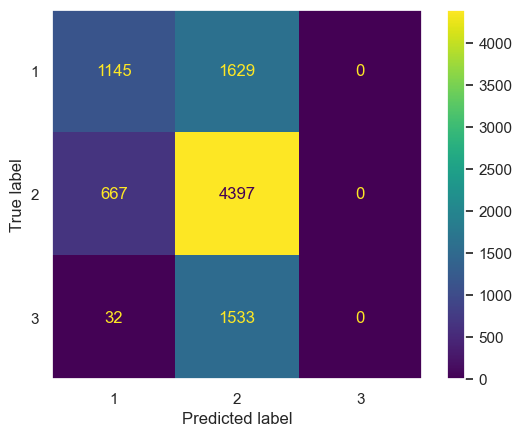
\includegraphics[width=\textwidth]{svmli.png}
    % \caption{Confusion matrix for SVM, linear kernel.}
    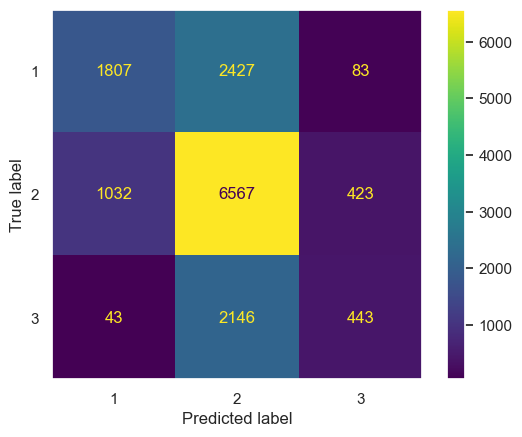
\includegraphics[width=\textwidth]{logisticWithOutliers.png}
    \caption{Logistic with outliers}
    % \label{fig:right}
\end{subfigure}
\caption{Confusion matrices for the models}
\end{figure}
\clearpage
\section*{Conclusion and discussion}

\newpage
\section*{References}
\textbf{Dataset}\\
https://www.kaggle.com/datasets/parisrohan/credit-score-classification/data
\vspace{5mm}\newline
\textbf{Literature Review}\\
% https://www.sciencedirect.com/science/article/pii/S1568494620302039
Dastile, X., Celik, T., \& Potsane, M. (2020).
Statistical and machine learning models in credit scoring: A systematic literature survey.
Applied Soft Computing, 91. doi:10.1016/j.asoc.2020.106263.
\vspace{5mm}\newline
% https://www.sciencedirect.com/science/article/abs/pii/S0377221721005695
Dumitrescu, E., Hué, S., Hurlin, C., \& Tokpavi, S. (2022). 
Machine learning for credit scoring: Improving logistic regression 
with non-linear decision-tree effects. European Journal of Operational 
Research, 297(3), 1178-1192. doi:10.1016/j.ejor.2021.06.053
%   talks about a modified logistic regression called "penalised 
%   logistic tree regression" that combines elements of decision trees and
%   logistic reg based on the adaptive lasso logistic regression model
% https://link.springer.com/chapter/10.1007/978-3-030-66891-4_5
% Guidolin, M., Pedio, M. (2021). Sharpening the Accuracy of Credit Scoring 
% Models with Machine Learning Algorithms. In: Consoli, S., Reforgiato Recupero, 
% D., Saisana, M. (eds) Data Science for Economics and Finance. Springer, Cham.
% https://doi.org/10.1007/978-3-030-66891-4\_5
% https://sci-hub.se/10.1057/jors.2009.129
% https://www.spglobal.com/marketintelligence/en/news-insights/blog/machine-learning-and-credit-risk-modelling
% Yue, Lei, and Luka Vidovic. “Machine Learning and Credit Risk Modelling.”
%  \textit{Machine Learning and Credit Risk Modelling $\vert$ S\&P Global Market Intelligence}, 
%  S\&P Global Market Intelligence, 30 Nov. 2020, 
%  www.spglobal.com/marketintelligence/en/news-insights/blog/machine-learning
%  -and-credit-risk-modelling. 
\end{document}


% some drafts:
% https://sci-hub.se/10.1057/jors.2009.129
% interesting paper on showing weaknesses of evaluation statistics. not sure if its
% all that relevant though
% Hand and Zhou observe the performances of nine supervised learning 
% classification models in classifying customers in retail banking and discuss how 
% different commonly used methods such as area under curve (AUC), Gini measures, Kolmogorov–Smirnov statistic (KS), 
% used in  evaluating performance may give misleading conclusions due to 
% fundamental weaknesses behind these methods. For example, the KS statistic concluded that classification 
% trees performed the best while AUC ranks the model near the bottom.\\